\section{Thri-kreen}
\Quote{This one does not speak with the quivering soft shells that lay about all night. This one might eat you, but never speak.}{Tu'tochuk}

\begin{figure*}[t!]
\centering
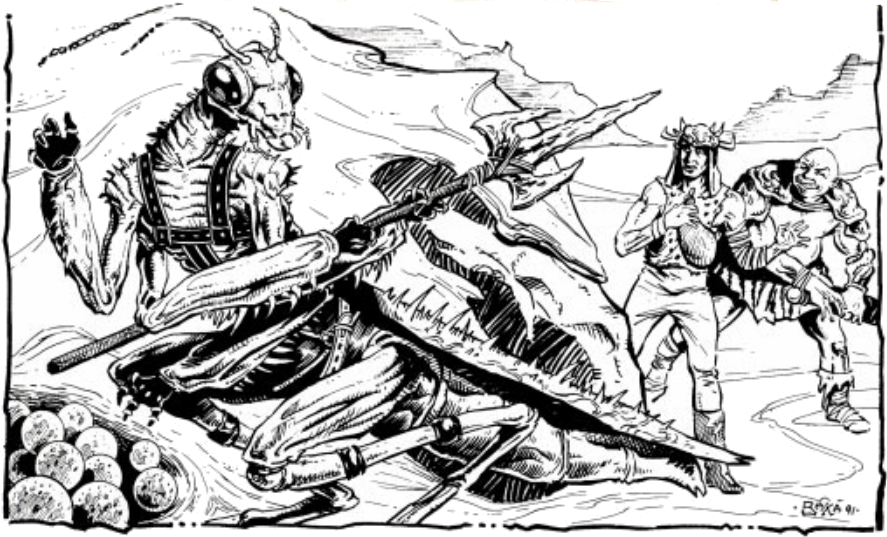
\includegraphics[width=\textwidth]{images/thrikreen-1.png}
\WOTC
\end{figure*}

Thri-kreen are the strangest of the intelligent races of the Tablelands. These insectoid beings possess a mindset very different from any humanoid being encountered. They roam the wastes in packs, hunting for food day and night, since they require no sleep. Thri-kreen are quick and agile and make fearsome fighters, feared throughout the wastes.

\textbf{Personality:} Since thri-kreen (also known simply as the kreen) do not require sleep, they have difficulty understanding this need in the humanoid races. They have difficulty understanding this state of ``laziness'' in others. Other behaviors of humanoids seem unnecessarily complex. A keen's life is simple: hunt prey. Kreen live for the hunt, and own only what they can carry.

\textbf{Physical Description:} Mature thri-kreen stand about 2.1 meters tall, with a rough body length of 3.3 meters. Their four arms end in claws; their two legs are extremely powerful, capable of incredible leaps. However, kreen are unable to jump backwards. Their body is covered with a sandy-yellow chitin, a tough exoskeleton that grants the thri-kreen protection from blows. Their head is topped with two antennae, and their two eyes are compound and multifaceted. The kreen mouth consists of small pincers. Male and female thri-kreen are physically indistinguishable. Thri-kreen usually do not wear clothing, but wear some sort of harness to carry weapons and food. Many wear leg or armbands, or bracelets. Some attach rings on different places on their chitin, though this requires careful work by a skilled artisan.

\textbf{Relations:} The pack mentality dominates a keen's relation with others. Kreen hunt in packs, small groups that assemble together. Kreen will hunt prey in the same region for a while, but move on before their prey has been depleted. A kreen that joins a group of humanoids will often try to establish dominance in the group. This can be disconcerting to those unaware of the keen's behavior, since establishing dominance usually means making threatening gestures. Once the matter is settled, they will abide by the outcome. Thri-kreen view humanoids as sources of food, though they don't usually hunt them, only in dire need. Many kreen have a particularly fond taste for elves; as such, meetings between these two races are often tense. However, once part of a clutch, thri-kreen will never turn on their humanoid friends, even in the worst of situations.

\textbf{Alignment:} Most thri-kreen are lawful, since the pack mentality is ingrained in their beings. Kreen that deviate from this mentality are rare.

\textbf{Kreen Lands:} No thri-kreen settlements exist in the Tyr region; kreen encountered there are either small packs of kreen, or else adventuring with humanoids. To the north of the Tyr region, beyond the Jagged Cliffs, past the Misty Border, lies the Kreen Empire. This great nation of kreen rules the Crimson Savanna, forming great city-states that rival the humanoid city-states of the Tyr region.

\textbf{Magic:} Thri-kreen have no natural disposition towards magic, and a wizard's use of the environment as a source of power conflicts with a keen's beliefs. As well, the keen's lack of sleep and its instinctual need to hunt do not lend themselves well to magical study. Kreen wizards are extremely rare: no one has ever seen one in the Tablelands.

\textbf{Psionics:} Kreen view psionics as a natural part of their existence. Some packs rely on telepathy to communicate with each member and coordinate their hunting abilities. Many kreen also use psionic powers to augment their already formidable combat prowess. Psychometabolic powers are often used to boost speed, metabolism or strength to gain an advantage in combat. Most kreen (even non-adventurers) take the psychic warrior class, which kreen consider a natural part of growing up. Kreen do not need instruction to advance in the psychic warrior class---it comes to them as part of their ancestral memory.

\textbf{Religion:} Thri-kreen have no devotion to any god, but they hold nature and the elements in high regard. Ancestral memories guide them through their lives. Thri-kreen revere the Great One, a legendary kreen leader from the past.

\textbf{Language:} The Kreen language is very different from those of the other intelligent races. They have no lips or tongues, and so cannot make the same sounds humanoids make. Kreen language is made up of clicks, pops, or grinding noises.

\textbf{Names:} Kachka, Ka'Cha, Ka'Ka'Kyl, Klik-Chaka'da, Sa'Relka, T'Chai

\textbf{Adventurers:} Kreen adventure for different reasons. Most enjoy challenges presented by new prey. Some seek out the challenge of leading new clutches, new companions and observing the different ``hunting'' techniques of the dra (sentient meat-creatures such as humans).

\subsection{Thri-Kreen Society}
Thri-kreen hatch from eggs. All those who hatch at the same time form what is called a clutch. Thri-kreen gather in packs that roam the wastes. Each pack consists of several clutches that roam over an area that the pack considers theirs to hunt on. There are no permanent thri-kreen communities.

Clutches and packs are organized along strict order of dominance. The toughest member is leader; the second most powerful is second in command and so forth. A thri-kreen can challenge a superior for dominance initiating a contest. The contestants fight until one surrenders or dies. Afterwards, the matter is considered settled and there are no lingering resentments between victor and loser. The pack-mates take the view that the challenger was only acting to strength the pack.

Thri-kreen are obsessed with hunting. They are carnivores, but seldom hunt intelligent life for food. They do have a taste for elf, which gives them a bad reputation amongst Elven tribes. When not hunting, they craft weapons, teach their young, and craft sculptures.

The pack mentality is so ingrained in the culture that thri-kreen apply it to every situation. Thri-kreen feel compelled to be part of a clutch and will accept members of other races as clutch-mates.

\subsection{Roleplaying Suggestions}
You tend to rely on your natural attacks and special kreen weapons. Everything you kill is a potential dinner. You have a strong need for a party leader - obedience to this leader in the party is important to you. If you seem to be the most powerful and capable, then you will assume leadership; if someone challenges your authority then you will wish to test whether they are in fact stronger than you. It is not a question of vanity; you won't want to fight to the death, but merely to ascertain who is worthy to lead the party. You do not have the focus of a dwarf to complete a project, but you would give your life to protect your companions. If you did not trust and honor them as your own family, then you would not travel with them and work together with them. You do not understand the concept of sleep. It disturbs you that your dra companions lie unconscious for a third of their lifetimes. You own only what you can carry, caring little for money or other items that other races consider as treasure. Your philosophy of ownership sometimes leads you into conflict with presumptuous dra who think they can own buildings, land, and even whole herds of cattle!


% \begin{figure*}[t!]
% \centering
% 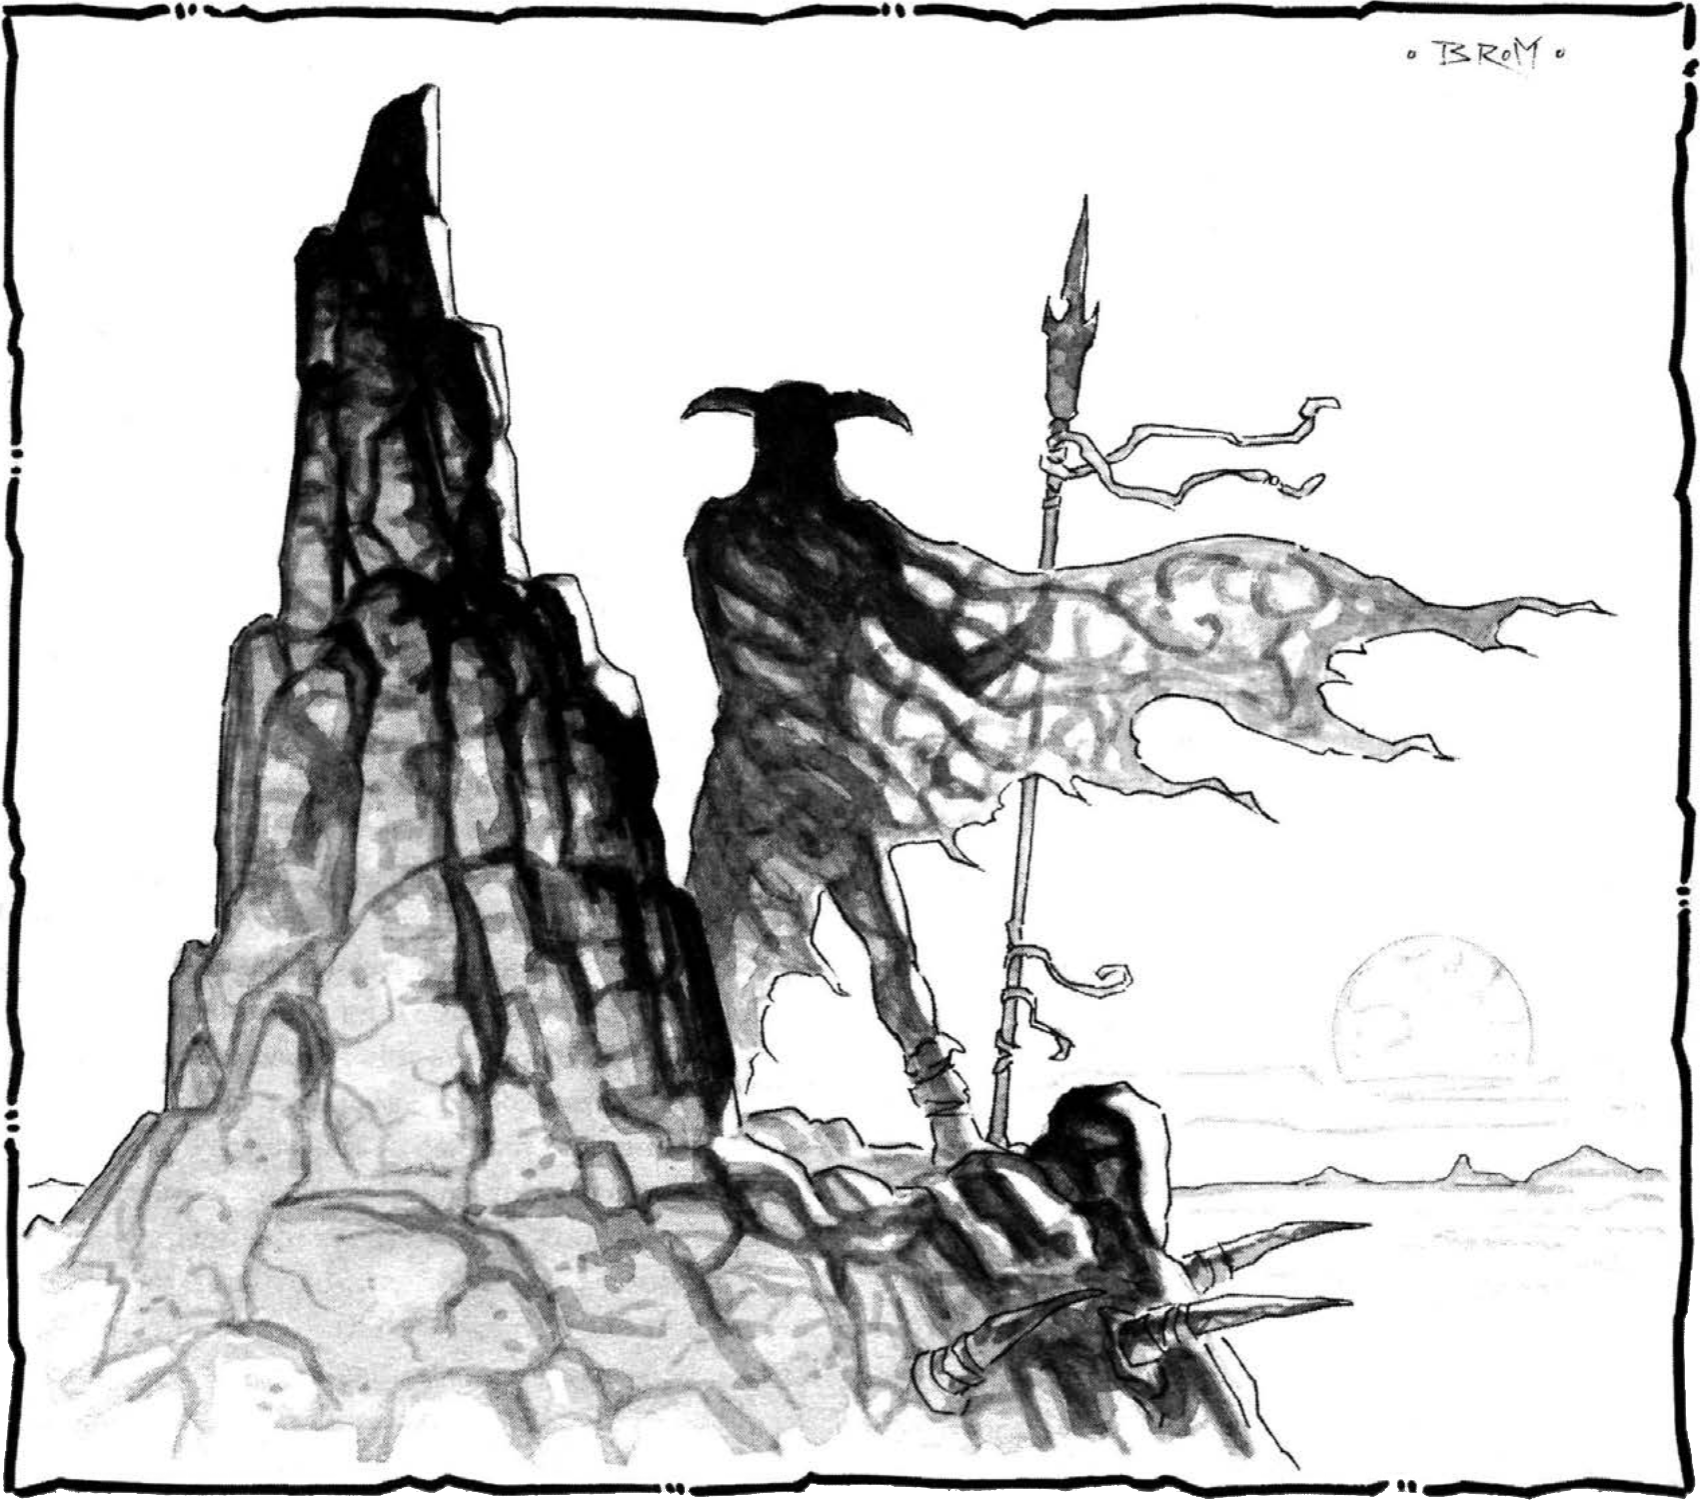
\includegraphics[width=\textwidth]{images/adventurer-2.png}
% \WOTC
% \vskip5mm
% \end{figure*}


\subsection{Thri-Kreen Racial Traits}
\begin{itemize*}
    \item +4 Dexterity, $-2$ Intelligence, +2 Wisdom, $-4$ Charisma: Thri-kreen are fast, but their alien mindset makes it difficult for them to relate to humanoids; furthermore, their ``clutch-mind'' instincts leave them with a poor sense of themselves as individuals.
    \item Monstrous Humanoid: Thri-kreen are not subject to spells or effects that affect humanoids only, such as \spell{charm person} or \spell{dominate person}.
    \item Medium: Thri-kreen receive no advantages or penalties due to size.
    \item Thri-kreen base land speed is 12 meters.
    \item Darkvision out to 18 meters.
    \item Sleep Immunity: Thri-kreen do not sleep, and are immune to sleep spells and similar effects. Thri-kreen spellcasters and manifesters still require 8 hours of rest before preparing spells or regaining power points.
    \item Natural Armor: Thri-kreen have a +2 natural armor bonus to AC due to their naturally tough and resistant chitin.
    \item Multiple Limbs: Thri-kreen have four arms, and thus can take the \feat{Multiweapon Fighting} feat instead of the \feat{Two-Weapon Fighting} feat. Thri-kreen can also take the \feat{Multiattack} feat. (These are not bonus feats.)
    \item Natural Weapons: Thri-kreen may make bite and claw attacks as a full round action. Their primary claw attack does 1d4 points of damage for each of their four claws. Their secondary bite attack, deals 1d4 points of damage, and has a chance to poison. A thri-kreen can attack with a weapon (or multiple weapons) at its normal attack bonus, and make either a bite or claw attack as a secondary attack.
    \item Deflect Arrows: Thri-kreen gain the benefit of the \feat{Deflect Arrows} feat.
    \item Leap (Ex): A thri-kreen with 3 or more Hit Dice become natural jumpers, gaining a +30 racial bonus to all \skill{Jump} checks.
    \item Poison (Ex): A thri-kreen with 5 or more Hit Dice delivers its poison with a successful bite attack. Fortitude DC 11 + Con modifier. The initial and secondary damages are paralysis for 1d10 rounds.
    \item Weapon Familiarity: To thri-kreen, the chatkcha and gythka are treated as martial rather than exotic weapons. These weapons are more common among thri-kreen than among other races.
    \item Thri kreen have a +4 racial bonus on \skill{Hide} checks in sandy or arid areas-.
    \item Alien Mind (Ex): A thri-kreen has difficulty understanding how the humanoid minds work. Whenever a thri-kreen targets a creature of another race with mind-affecting abilities, that creature gains +1 to its save against those powers.
    \item Automatic Languages: Kreen. Bonus Languages: Common, Dwarven, Elven, Entomic, Saurian, and Terran.
    \item Favored Class: Druid or Fighter. A thri-kreen must choose between druid or fighter as favored class. This choice cannot be changed. A multiclass thri-kreen's chosen class does not count when determining whether he takes an experience point for multiclassing.
    \item Level Adjustment: +2.
\end{itemize*}
